\section{Serveis per particulars i aficionats a la genealogia}

    \paragraph{}
    A part dels serveis per organitzacions, FamilySearch disposa d'un ampli ventall d'eines i funcionalitats pels genealogistes amateurs o aficionats. Aquestes eines es poden dividir en dos grans blocs. El bloc encarregat de gestionar la informació genealògica dels usuaris i el bloc de cerca sobre les bases de dades de FamilySearch.

    Les eines de gestió sobre la informació genealògica particular, permeten als usuaris digitalitzar la seva informació d'una forma fàcil, estructurada i accessible, que com\-pleix amb els estàndards del sector.

    Per altra banda, les eines de cerca constitueixen el principal atractiu de l’or\-ga\-nit\-za\-ció per particulars i aficionats a la genealogia. Aquest conjunt d'eines han estat pensades per l’exploració de les dades emmagatzemades en l'ampli catàleg de registres de FamilySearch.

    Finalment, FamilySearch també permet, a aquelles persones interessades, formar part d'un encadenat de voluntaris lligat a l'organització, encarregat d'ajudar, coordinar i arbitrar, el procés d'indexació dels registres genealògics.


    \subsection{Eines genealògiques}

    \paragraph{}
    El primer bloc d'eines al que fèiem referència en la introducció, eren el conjunt d'eines encarregades de la manipulació de la informació genealògica per particulars. Les eines principals giren al voltant de la creació d’arbres genealògics i un conjunt d'opcions per adjuntar fonts d’informació, arxius multimèdia i altres menes de docu\-ments.

    Actualment, existeixen moltes eines que satisfan aquesta mateixa necessitat, tant en línia com aplicacions per escriptori i mòbil. Tanmateix, no són moltes les que ofereixen la possibilitat de complementar la informació coneguda pels usuaris amb re\-gis\-tres i informació ja disponible en el núvol.

    Dins d’aquest grup més reduït, destaquen \emph{Ancestry.com} i \emph{FamilySearch.org}, on només la darrera és d’accés gratuït. El conjunt de funcionalitats que destaquen per part de FamilySearch, es detallen breument a continuació.


    \subsubsection{Arbre familiar}

    \paragraph{}
    Dins de l’estudi de la genealogia, els arbres genealògics o arbres familiars solen ser l’element visual més conegut i utilitzat per representar la història i lligams familiars d'un individu.

    Els arbres familiars a FamilySearch són creats mitjançant les relacions de pa\-ren\-tesc entre diferents persones. Aquest fet és important, ja que FamilySearch demana crear aquestes persones per tal d'incorporar-les a les seves bases de dades. Aquestes persones seran públiques a menys que s'especifiqui que volen ser utilitzades de forma privada.

    La peculiaritat de FamilySearch és que quan es crea una nova persona, es busca en el sistema persones que podrien encaixar amb la persona proporcionada. D'aquesta forma, es redueix la creació de persones duplicades i inclús, a vegades, la informació coneguda pot ser complementada amb la ja existent a l'arbre familiar de FamilySearch.

    Un exemple d'arbre familiar de FamilySearch  pot ser visualitzat en la figura~\ref{fig:familyTree}.

    \begin{figure}[h]
        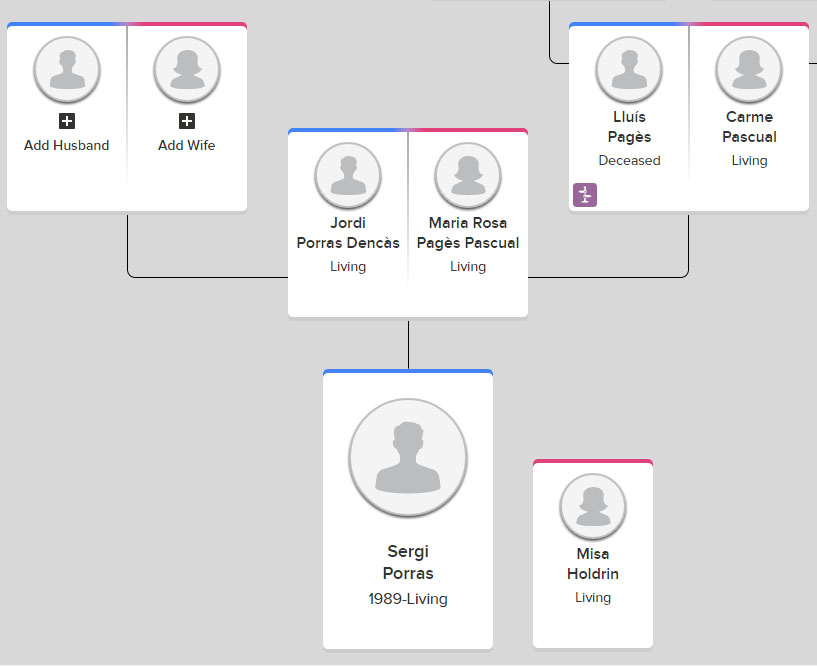
\includegraphics[scale=0.4]{03/familyTree}
        \centering
        \caption{Exemple d'arbre familiar.\label{fig:familyTree}}
    \end{figure}


    \subsubsection{Fan chart}

    \paragraph{}
    El Fan chart, o gràfic en forma de ventall, ofereix la possibilitat de visualitzar l'arbre familiar d'una persona de forma més compacta. Aquest format ofereix una visió de 360 graus sobre l'ascendència de la persona i la de la seva parella, però no inclou informació sobre la seva descendència.

    Oferim un exemple d’aquesta visualització en la figura~\ref{fig:fanChart}.

    \begin{figure}[h]
        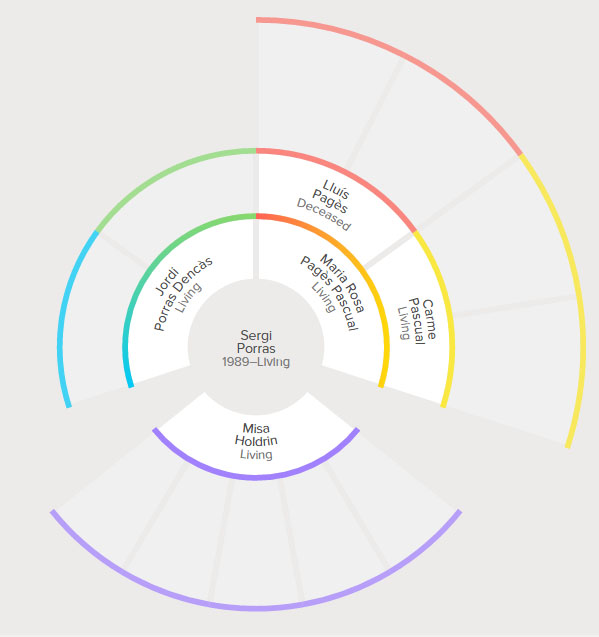
\includegraphics[scale=0.4]{03/fanChart}
        \centering
        \caption{Exemple de Fan Chart.\label{fig:fanChart}}
    \end{figure}


    \subsubsection{Detalls personals}

    \paragraph{}
    Una altra característica de les eines genealògiques és la capacitat de complementar la informació ge\-nea\-lò\-gi\-ca d'un usuari amb informació personal o informació ge\-nea\-lò\-gi\-ca més detallada.

    El conjunt d'informació extra que pot ser introduïda, s'exposa a continuació:

    \begin{itemize}
        \item \textbf{Esbós de la vida d'una persona:} Resum, d’estructura narrativa, que detalla com va viure la persona i quines van ser les diferents etapes de la seva vida.
        \item \textbf{Informació vital:} Gran part d’aquesta informació és la que ja s’ha introduït en el moment de crear la persona a l’arbre genealògic. Aquesta secció permet editar-la i afegir esdeveniments importants en la vida d’una persona, més enllà de la informació bàsica de naixement o defunció.
        \item \textbf{Fonts d’informació:} Permet introduir informació relacionada a les fonts d’informació que contrasten i validen la informació introduïda sobre la persona.
        \item \textbf{Discussions:} Les discussions són conversacions que poden obrir els usuaris per tal de discutir sobre la informació relativa a una persona.
        \item \textbf{Notes:} Les notes permeten anotar detalls concrets o informació extra que no té sentit dins de cap altre apartat.
    \end{itemize}


    \subsubsection{Memòries}

    \paragraph{}
    Les memòries són en gran part contingut multimèdia que els usuaris poden penjar i relacionar amb les persones de l'arbre familiar, per tal d'aportar informació personal extra sobre aquestes.

    Si recordem la definició de genealogia, aquesta no tractava només sobre l'estudi dels llinatges familiars, sinó també sobre l'estudi de com van viure aquestes persones. Aquest conjunt d'arxius multimèdia permet complementar la informació genealògica coneguda, amb informació que ajudi a comprendre qui van ser aquestes persones o que va caracteritzar la seva vida.

    FamilySearch suporta quatre tipus d'artefactes diferents. A continuació, s'explica en més detall en que consisteix cada un d'ells:

    \begin{itemize}
        \item \textbf{Fotografies:} Les fotografies representen la ciència o art encarregat de crear imatges perdurables en el temps de persones, moments o esdeveniments. Aquest artefacte permet relacionar fotografies a una persona de l'arbre familiar.
        \item \textbf{Documents:} Els documents solen ser fitxers PDF que proporcionen informació extra sobre aspectes concrets de la persona. Per exemple, un testament.
        \item \textbf{Notes de veu:} Les notes de veu són arxius d’àudio que els usuaris relacionen amb la vida d’una persona en qüestió. Un exemple podria ser, per exemple, un missatge de contestador o gravació auditiva.
        \item \textbf{Històries:} Les històries són peces narratives que els usuaris poden escriure per relatar les vivències d'una persona o documents escrits per la mateixa persona representada a l'arbre familiar.
    \end{itemize}


    \subsubsection{Family Booklet}

    \paragraph{}
    El Family Booklet és en un document que FamilySearch crea sota petició i que recopila tota la informació disponible relacionada amb la família de la persona que el sol·licita. Aquesta informació s'utilitza per crear un petit llibret que pot ser encarregat en format físic o descarregat digitalment.
